\begin{frame}
  \frametitle{Applications of the algorithm presented}
  \begin{columns}
    \begin{column}{0.5\textwidth}
    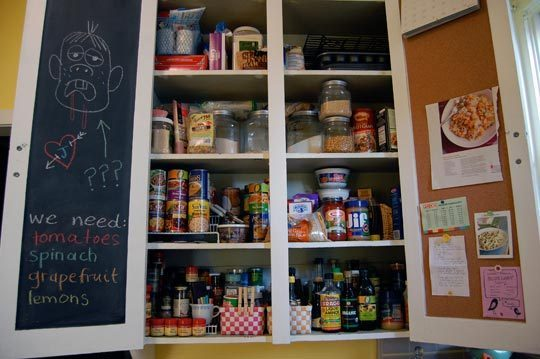
\includegraphics[width=\textwidth]{img/cupboard.jpg}

    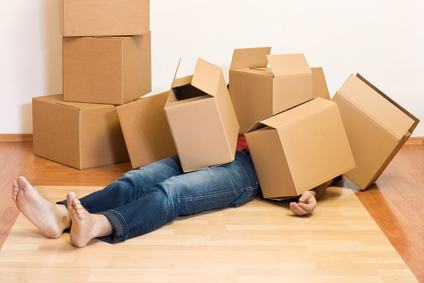
\includegraphics[width=\textwidth]{img/boxes.jpg}
    \end{column}
    \begin{column}{0.5\textwidth}
    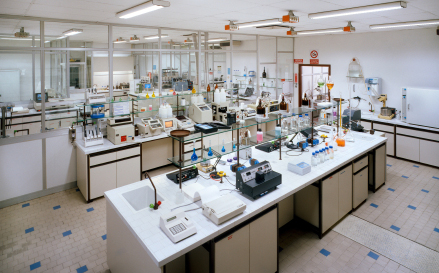
\includegraphics[width=\textwidth]{img/laboratory.jpg}

    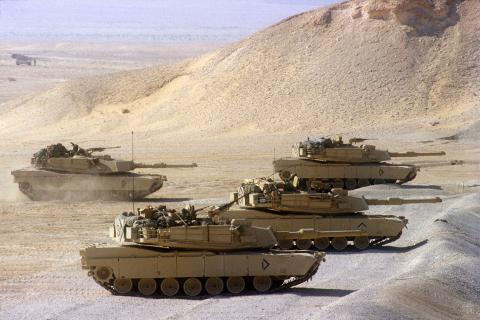
\includegraphics[width=\textwidth]{img/tanks.jpg}
    \end{column}
  \end{columns}
\end{frame}

\begin{frame}
  \frametitle{Applications of the general techniques learned}
  \begin{itemize}
    \item The Bayesian update is the same fundamental process as SLAM
  \end{itemize}
\end{frame}
